\chapter{Experiments}
\label{chap:experiments}
This chapter explains how the models were trained in order to obtain the best performances and an explanation map.
\section{Training}
Training of the models was done using the Adam\cite{kingma2014adam} optimizer and the pytorch\cite{pytorch_paszke2017automatic} library. An implementation in tensorflow\cite{tensorflow_45166} has been done but PyTorch was chosen as we needed to explain the model using the fullGrad\cite{fullgradient} GitHub repository. For the loss we chose Binary Cross Entropy as the task we are solving is a binary classification.

Training the different models required to fine turn some hyperparameter. Figure~\ref{fig:fine_tune_learning_rate} shows how the test loss can be used to compare the performances of the model when trained with different learning rates. Here we see that choosing a learning rate of \num{5e-05} seems to be the best decision to train the model. 

\begin{figure*}
    \centering
    \begin{subfigure}[b]{0.475\textwidth}
        \centering
        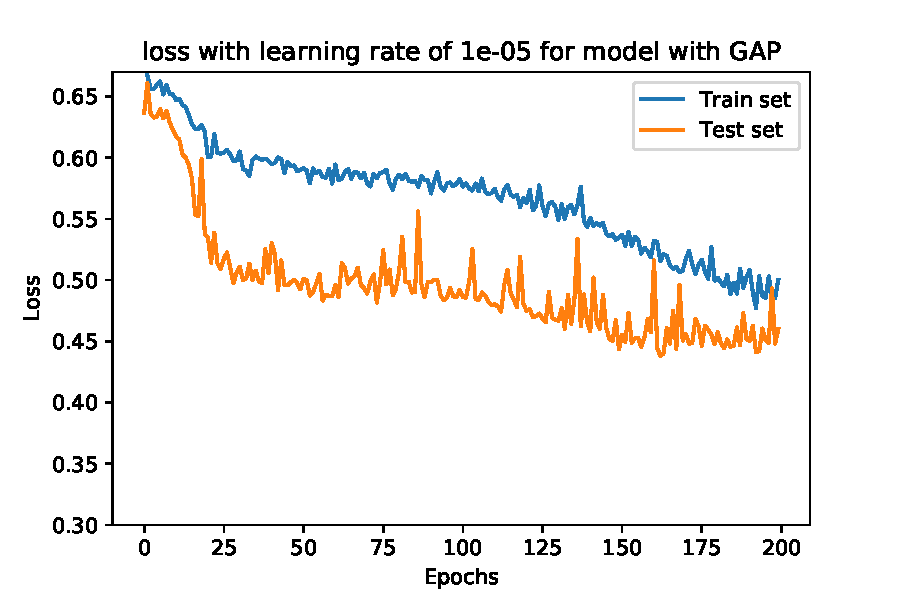
\includegraphics[width=\textwidth]{figures/Experiements/training_3D_CNN_GAP_lr_1e-05.pdf}
        \caption[Network2]%
        {{\small lr=\num{1e-05}}}    
    \end{subfigure}
    \hfill
    \begin{subfigure}[b]{0.475\textwidth}  
        \centering 
        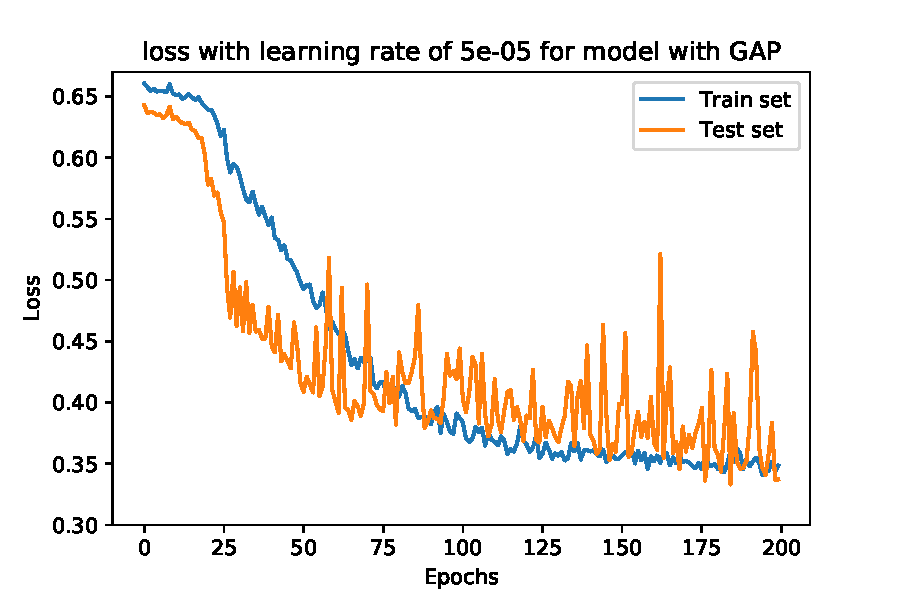
\includegraphics[width=\textwidth]{figures/Experiements/training_3D_CNN_GAP_lr_5e-05.pdf}
        \caption[]%
        {{\small lr=\num{5e-05}}}    
        \label{fig:best_lr}
    \end{subfigure}
    \vskip\baselineskip
    \begin{subfigure}[b]{0.475\textwidth}   
        \centering 
        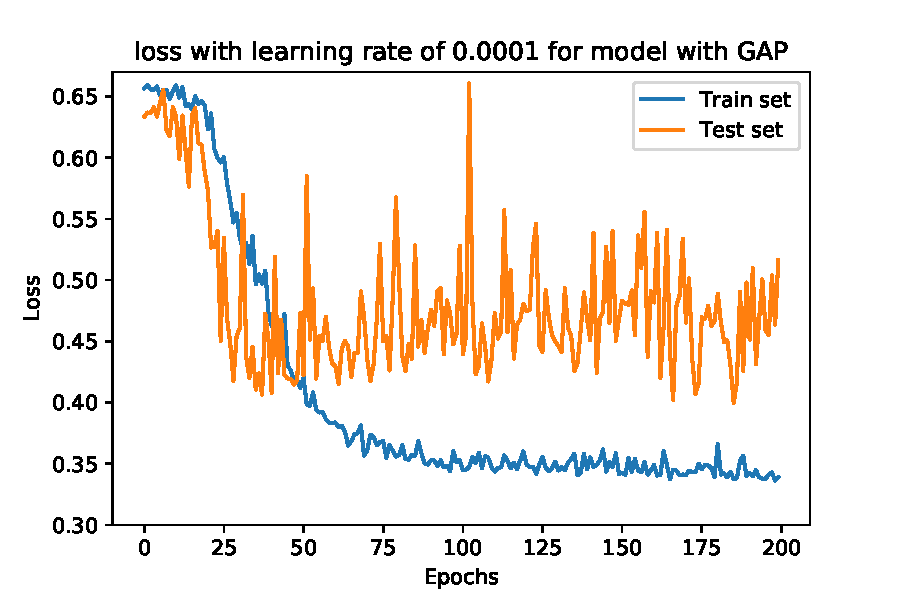
\includegraphics[width=\textwidth]{figures/Experiements/training_3D_CNN_GAP_lr_0.0001.pdf}
        \caption[]%
        {{\small lr=0.0001}}    
    \end{subfigure}
    \quad
    \begin{subfigure}[b]{0.475\textwidth}   
        \centering 
        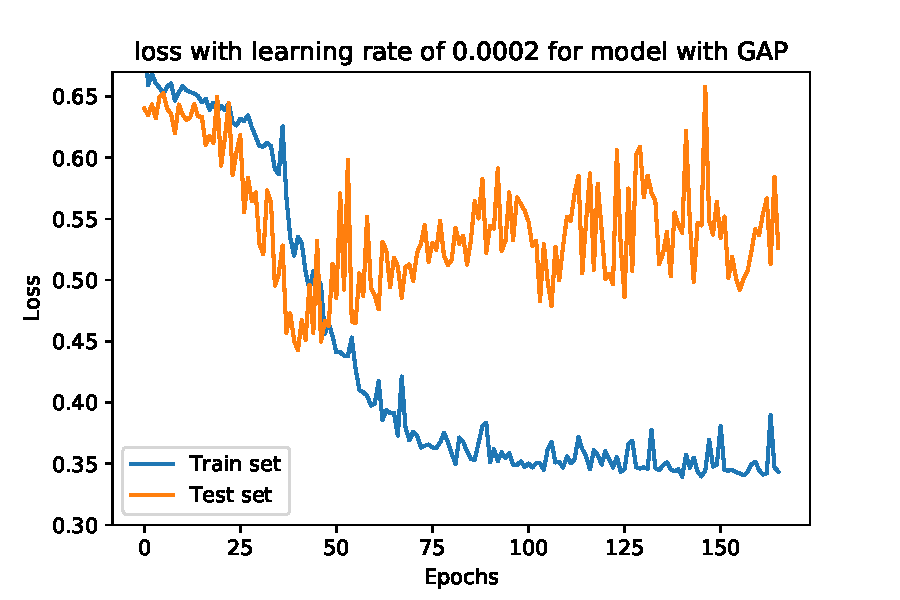
\includegraphics[width=\textwidth]{figures/Experiements/training_3D_CNN_GAP_lr_0.0002.pdf}
        \caption[]%
        {{\small lr=0.0002}}    
    \end{subfigure}
    \caption[ The average and standard deviation of critical parameters ]
    {\small Comparison of the train and test loss for different learning rate across 200 epochs of training. } 
    \label{fig:fine_tune_learning_rate}
\end{figure*}

Once trained, a network should be able to predict the correct class for any input. Unfortunately, the prediction of a model cannot be blindly trust. Nonetheless, the output of the network can be interpreted as a confidence score on the prediction of the network. Therefore even in the case where the network outputs $0.45$, which means that the patient does not have dementia, it can still be worth double-checking his case. In fact, for this particular prediction, the network is not so confident and has more chances of being wrong. Unfortunately, when trained for too long, the network tends to become overconfident and its outputs become almost binary (values close to zero or close to one), losing part of its interpretability. Label Smoothing \cite{label_smoothing_szegedy2015rethinking} aims at reducing the overconfidence of the network by changing the label of the train set from $0$ to $0 + \epsilon$ and from $1$ to $1 - \epsilon$. For the experiments, we chose $\epsilon$ to be $0.1$.

The loss used for training is Binary Cross Entropy. But as shown in figure~\ref{fig:OASIS_CDR_table} the data we are training on is unbalanced. Instead of training the model with the standard binary cross-entropy loss as defined in section~\ref{sec:binary_cross_entropy}, we used a variant that penalizes more the mistakes made on the underrepresented class. In our case, as we have approximately 70 percent of control samples and 30 percent of samples from people with dementia, the loss for a demented sample would be weighted by $\frac{1}{0.3} = 3.33$ and the other by $\frac{1}{0.7} = 1.43$.

Note that more could have been done in order to better train the model such as trying another optimizer or even using a learning rate scheduler, but we preferred to focus on explainability instead of performances.

\section{Evaluation}
The performance of the different model being very similar, we will perform the evaluation on the standard convolution model described in section~\ref{sec:standard_cnn}. This section purely evaluates the model's performance and resistance to age bias but is not interested in the explainability of the model. 


\subsection{Bias due to age}
\begin{wrapfigure}{r}{0.6\textwidth}
 \centering
 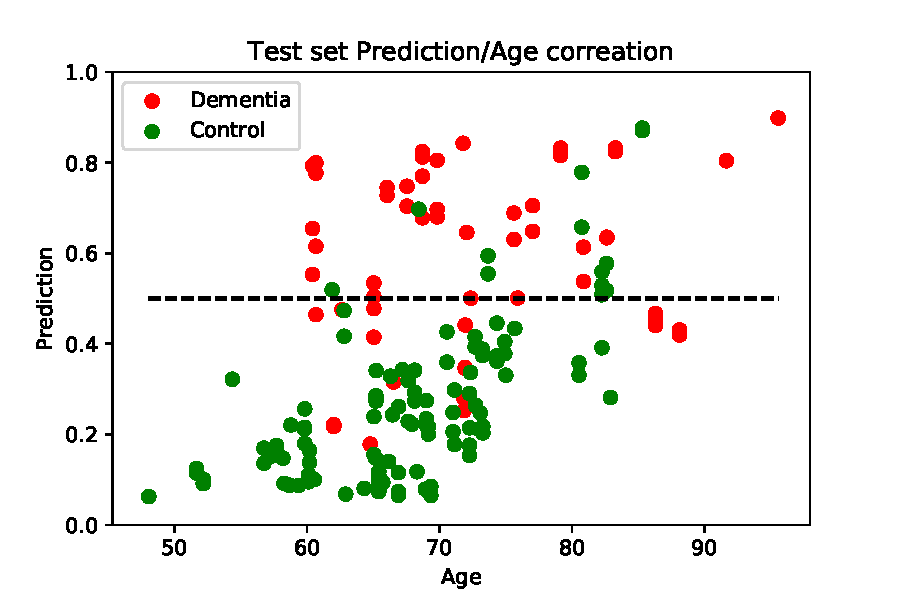
\includegraphics[width=.9\linewidth]{figures/Experiements/Eval/prediction_age.pdf}
 \captionsetup{width=.9\linewidth}
 \caption[PredPerAge]{Prediction of dementia per age.}
 \label{fig:prediction_per_age}
\end{wrapfigure}
As shown in the section~\ref{sec:OASIS}, the OASIS dataset presents a bias to age. To evaluate the model bias we can look at figure~\ref{fig:prediction_per_age}. We can see a trend that the model tends to more easily predict dementia to an old person than a young one.


\subsection{Metrics}
In order to evaluate and compare the different model, we used the metrics defined in section~\ref{sec:losses_metrics}. The confusion matrix in figure~\ref{fig:test_conf_matrix} allows us to compute the accuracy which is of $81.87\%$. This metric is quite confusing as it seems to be a good performance, but random guessing already has an accuracy of $70.76\%$. Instead, we can compute the precision which is of $74\%$ and the recall to be of $67.27\%$.

Figure~\ref{fig:roc_and_pr_curve} shows the ROC and PR curves to gain a better sense of the model performance. Note that as the dataset is unbalanced it is recommended to look at the PR curve. 

\begin{wrapfigure}{r}{0.6\textwidth}
 \centering
 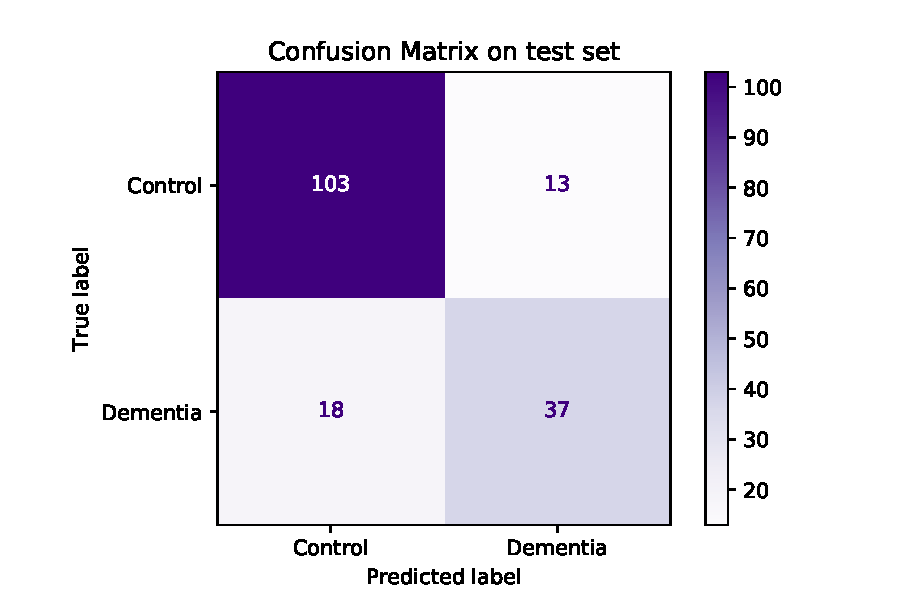
\includegraphics[width=.9\linewidth]{figures/Experiements/Eval/test_confusion_matrix.pdf}
 \captionsetup{width=.9\linewidth}
 \caption[ConfMatrix]{Confusion Matrix on the test set.}
 \label{fig:test_conf_matrix}
\end{wrapfigure}


\begin{figure}
\centering
\begin{subfigure}{.5\textwidth}
  \centering
  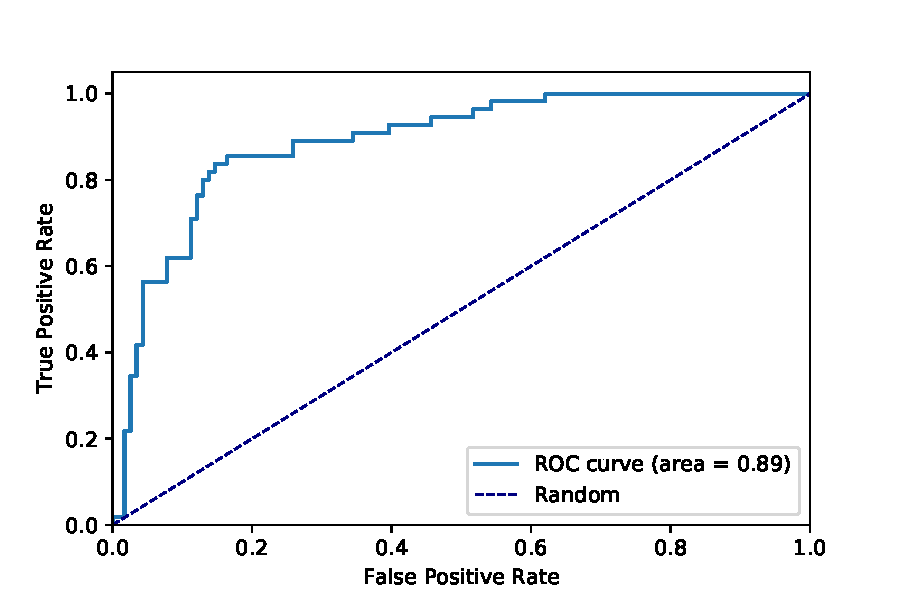
\includegraphics[width=1\linewidth]{figures/Experiements/Eval/ROC_curve.pdf}
  \caption{ROC curve.}
  \label{fig:roc_curve}
\end{subfigure}%
\begin{subfigure}{.5\textwidth}
  \centering
  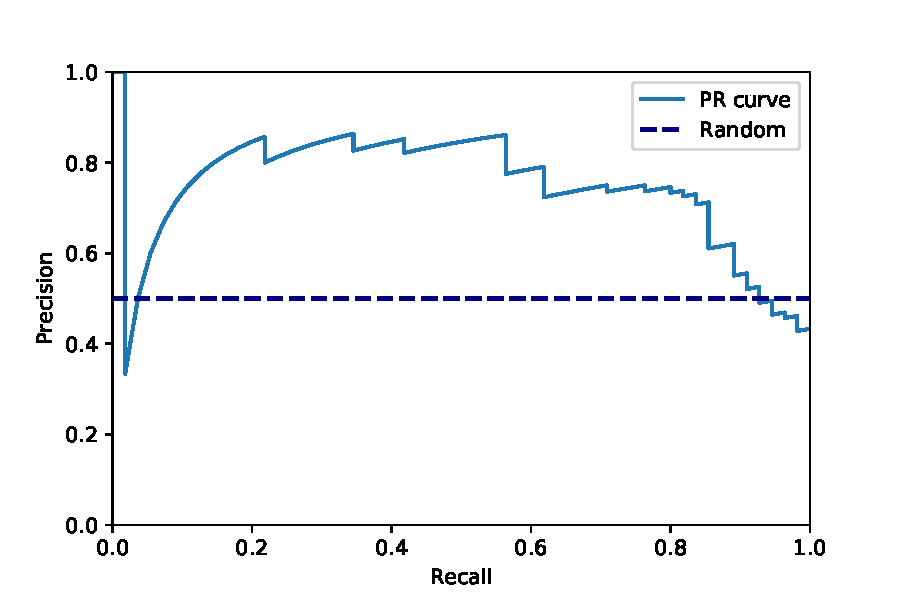
\includegraphics[width=1\linewidth]{figures/Experiements/Eval/pr_curve_curve.pdf}
  \caption{Precision and Recall curve.}
  \label{fig:pr_curve}
\end{subfigure}
\caption[Curve]{Evaluation curves.}
\label{fig:roc_and_pr_curve}
\end{figure}

\newpage
\section{Model Output Explanation}

As shown in figure~\ref{fig:alzheimerbrain}, Alzheimer disease tends to severely damage some specific regions of the brain. One of these regions is the hippocampus which serves at the creation of new memories. We would expect from a good explainer that indeed it highlights this specific region when explaining the output for a damaged brain. Figure~\ref{fig:dem_vs_control_age_pred} compares the outputs of the 3 algorithms we implemented on different slices of a damaged brain. In fact, in figure~\ref{fig:explainer_compared} we chose slices where the hippocampus is visible and observed that while Shap explanation is difficult to interpret, both GradCam and FullGrad focus on the hippocampus. It is especially visible with the output of the fullgrad algorithm where its maximal attention on this slice is actually located inside the hippocampus. For the rest of the report, we chose to work with fullgrad as its output makes more sense to us and is also sharper. The brain viewer implemented in annex~\ref{chap:brainviewer} is designed to work with a fullgrad saliency map.

Looking at the fullgrad output in figure~\ref{fig:fullgrad_output}, it is also interesting to see the focus that the model has on the ventricles that typically grows larger for damage brains. 



\begin{figure}
    \centering
    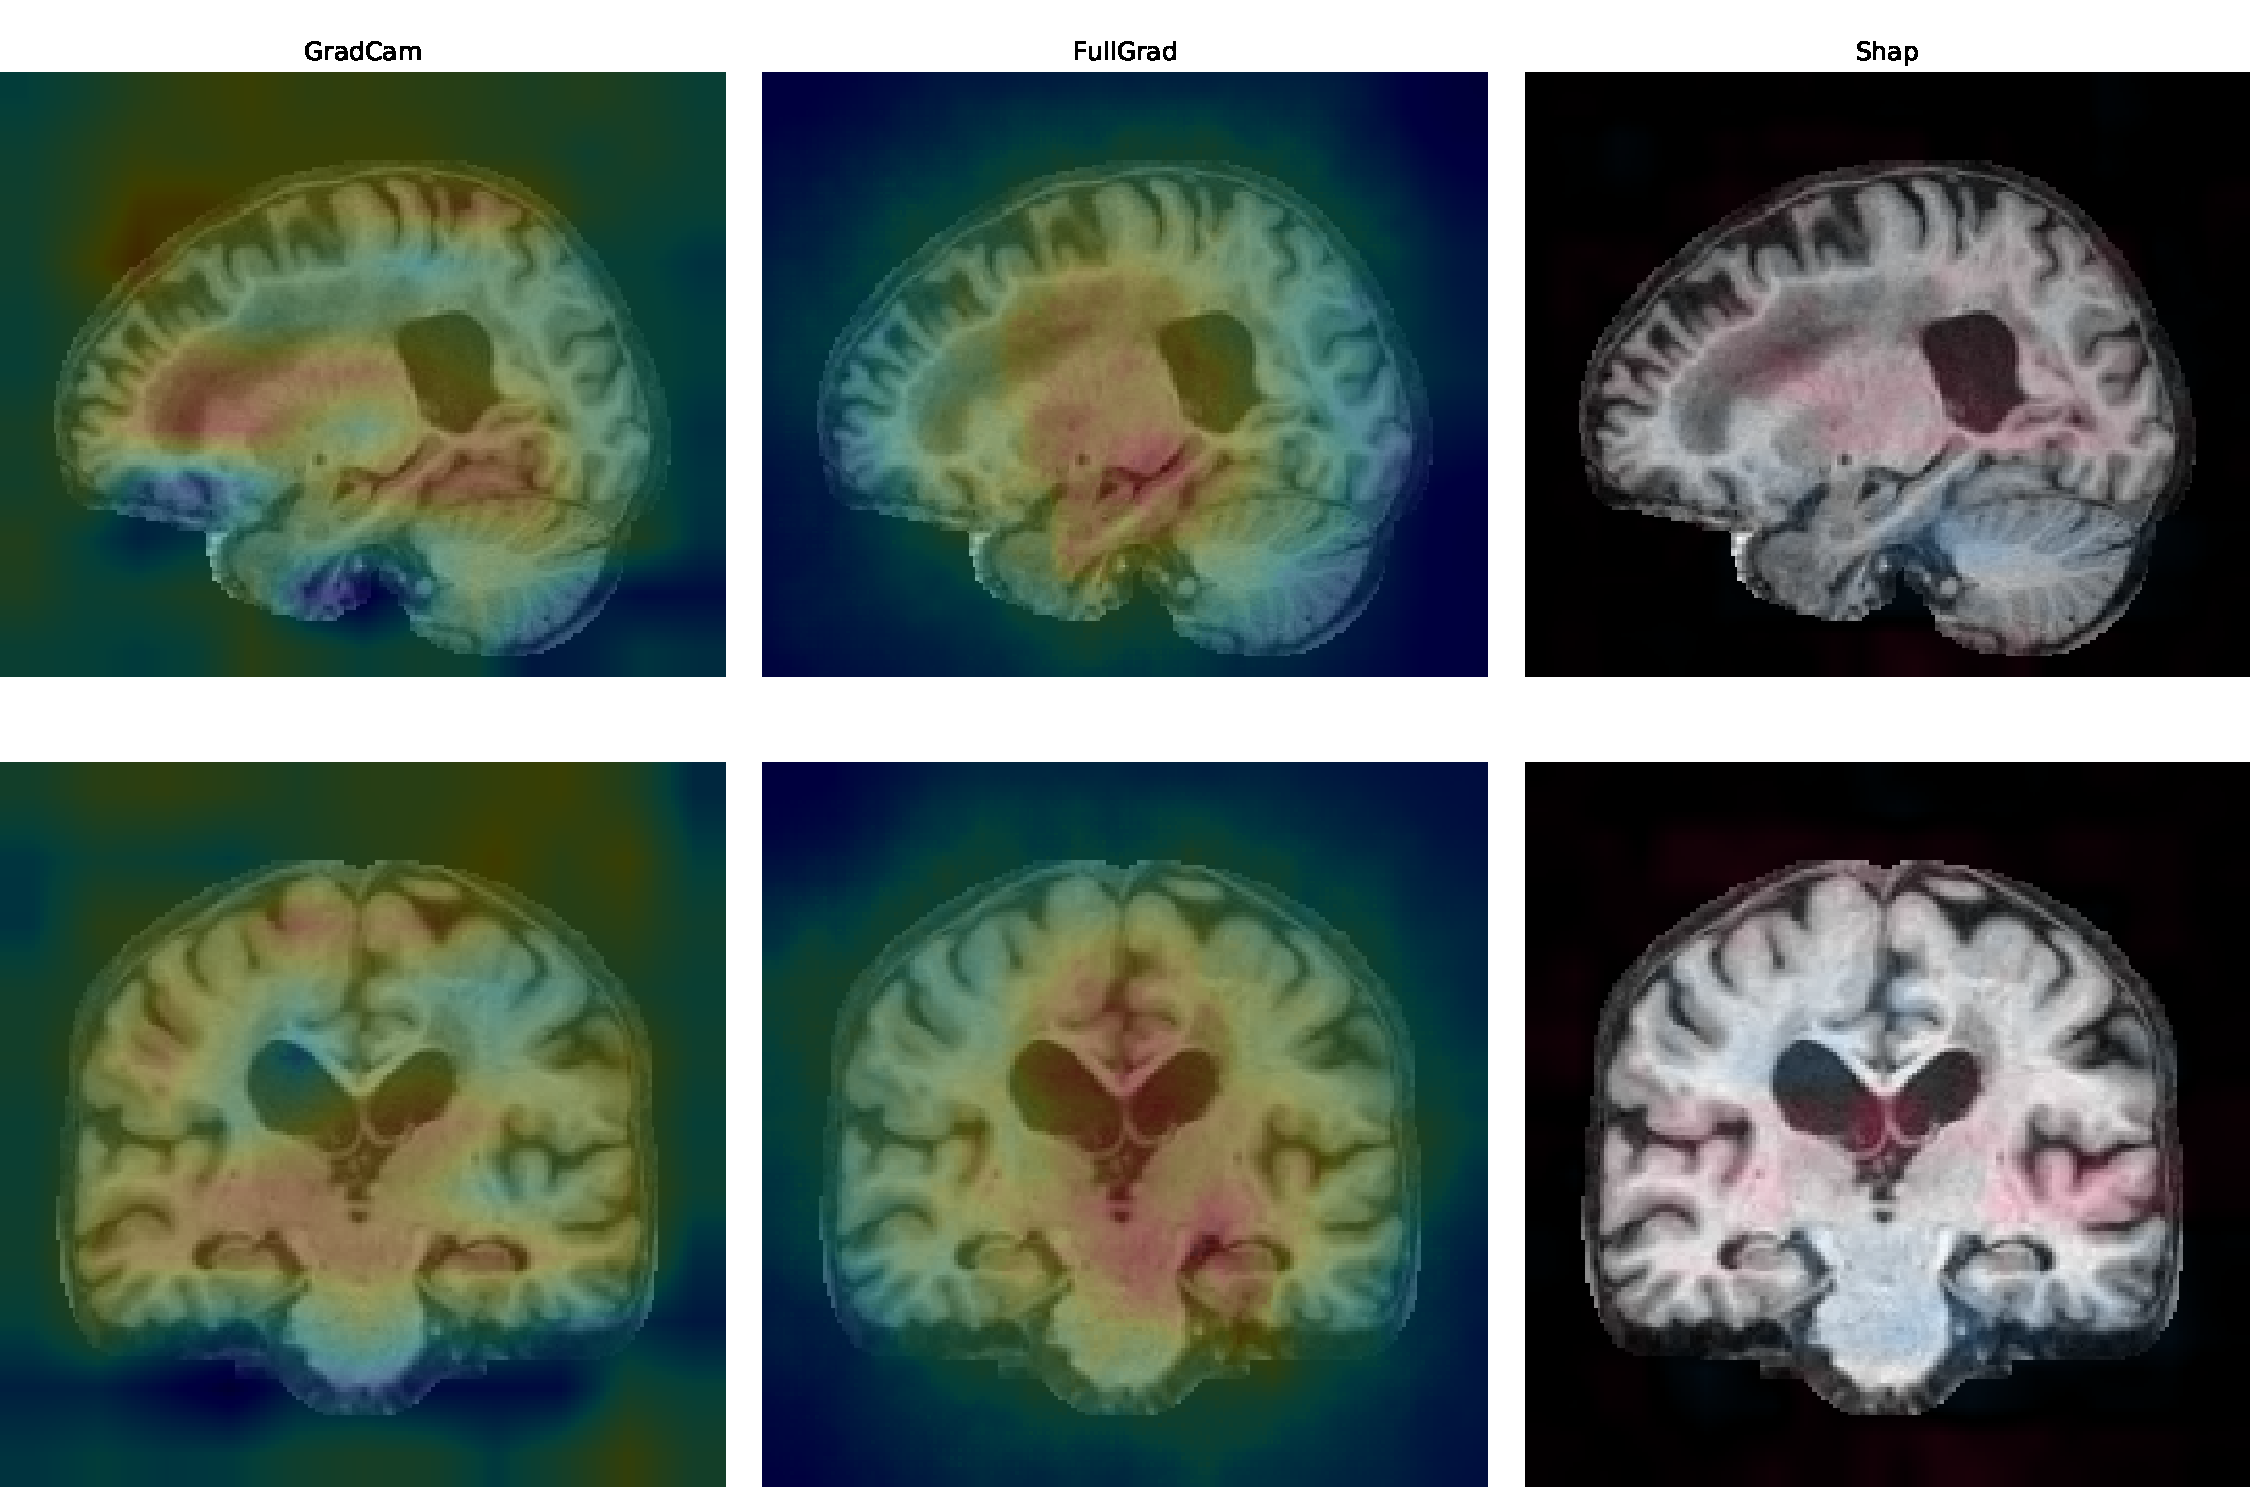
\includegraphics[width=0.9\linewidth]{figures/Experiements/explainer_coparaison.pdf}
    \caption{Outputs of the explainer algorithm on one patient with dementia.}
    \label{fig:explainer_compared}
\end{figure}

\begin{figure}
    \centering
    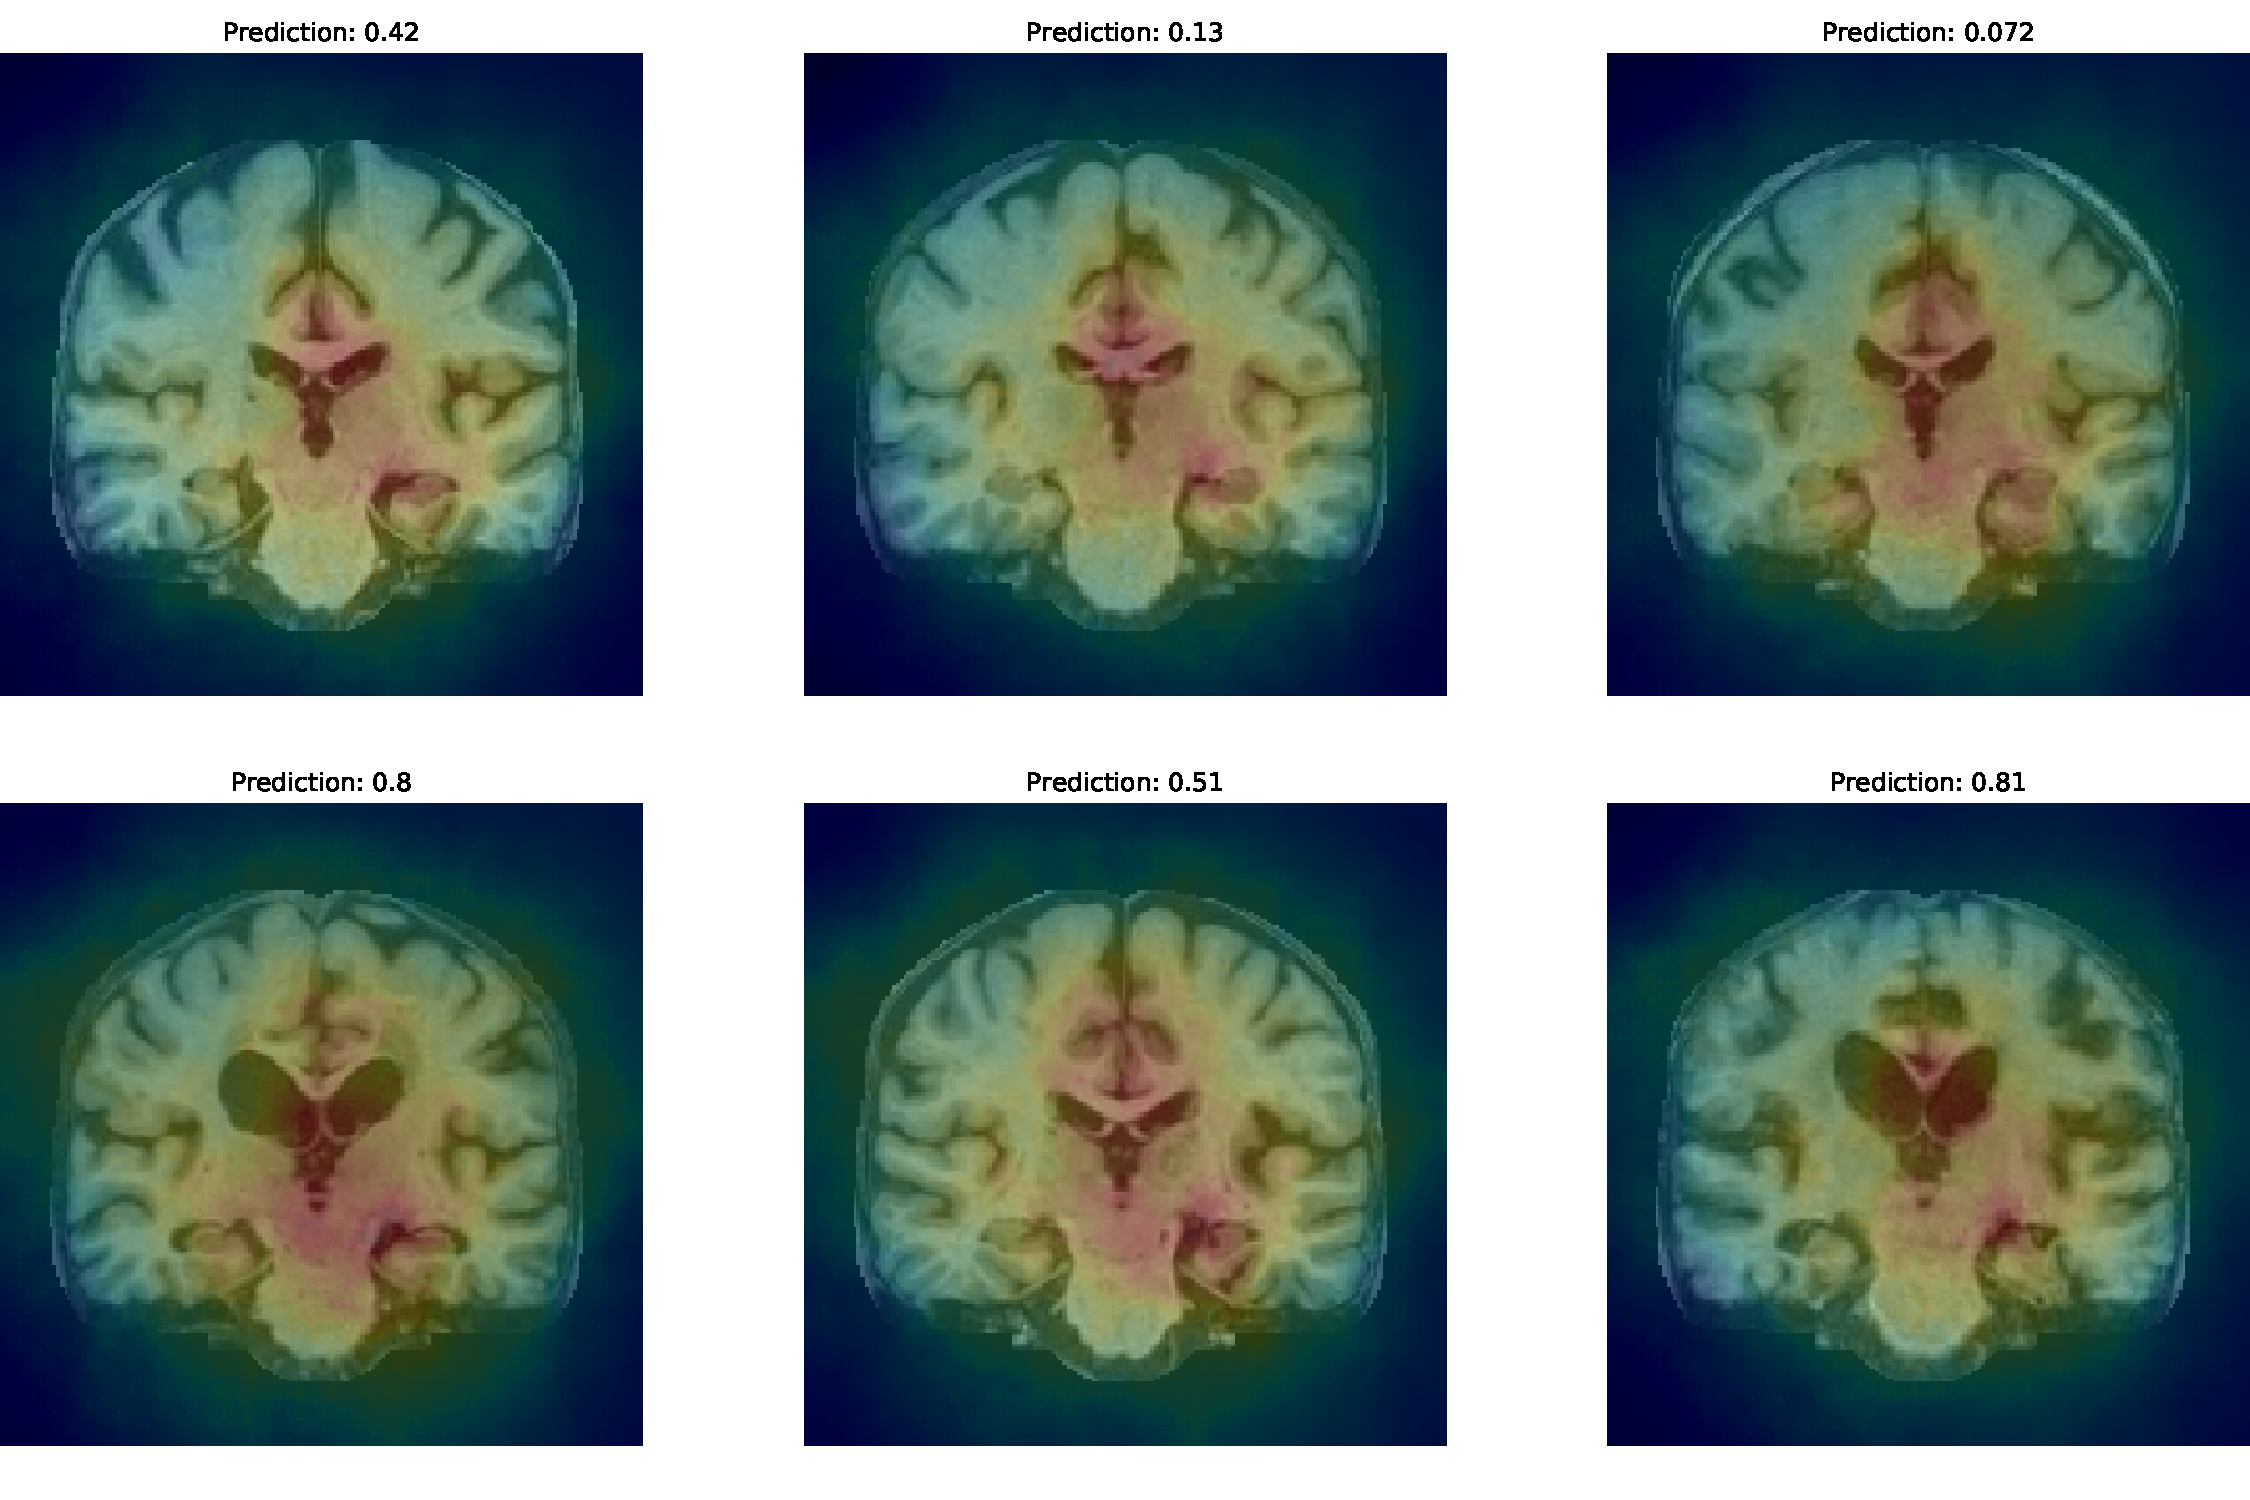
\includegraphics[width=1\linewidth]{figures/Experiements/output_fullgrad.pdf}
    \caption{Outputs of the fullgrad algorithm,the first row is composed of control patients and the second one of dementia patients. }
    \label{fig:fullgrad_output}
\end{figure}